\section{Solución Propuesta}

    En la figura \ref{fig:Diagrama} se observa un diagrama del \gls{sistema} propuesto donde se destacan las interacciones del sistema. Se inicia con un objeto del mundo real que es observado por el sensor Kinect, el cual obtiene imagen RGB, infrarroja y las distancias de una matriz de puntos, que pasan por un preprocesamiento para eliminar datos no deseados; usando un algoritmo de reconocimiento se obtiene la aproximación del objeto a una figura simple la cual es mostrada en un ambiente virtual creado en la computadora.\\
    
    
    \begin{figure}[!htb] 
        \centering
        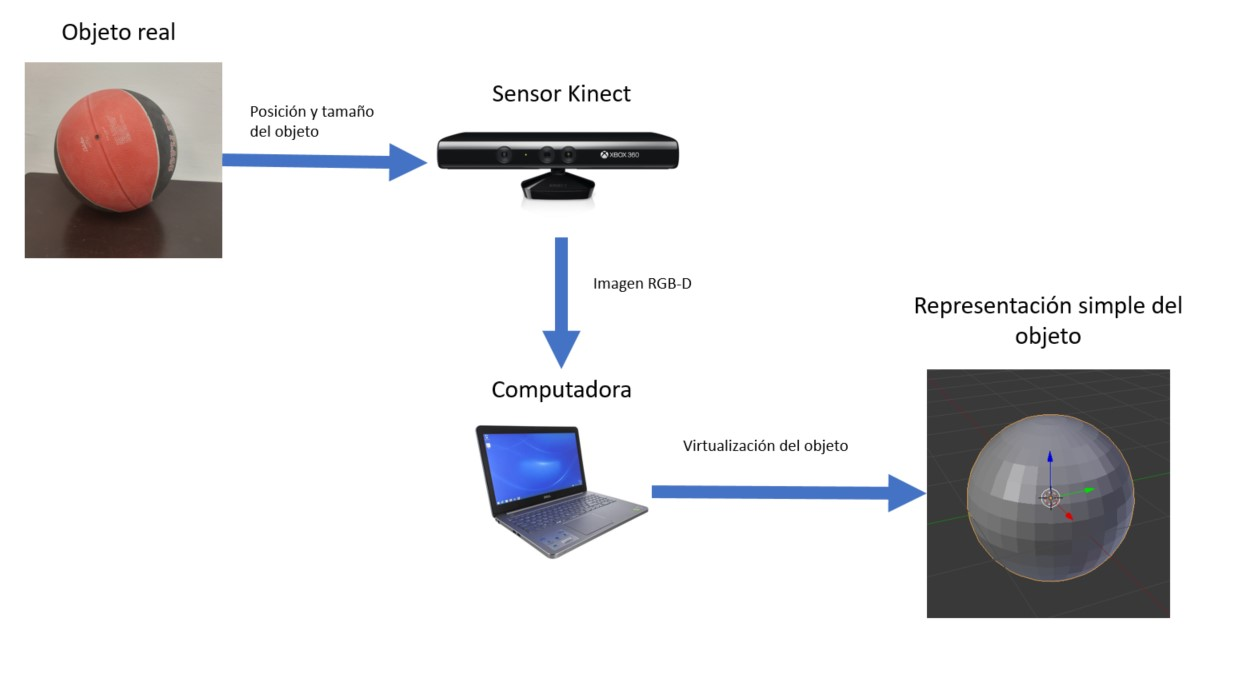
\includegraphics[width=\textwidth]{01Introduccion/imagenes/Diagrama_del_sistema.jpg}
        \caption{Diagrama del sistema propuesto} 
        \label{fig:Diagrama}
    \end{figure} 
